
%(BEGIN_QUESTION)
% Copyright 2008, Tony R. Kuphaldt, released under the Creative Commons Attribution License (v 1.0)
% This means you may do almost anything with this work of mine, so long as you give me proper credit

Sketch a circuit whereby this loop-powered pressure transmitter sends a signal to an analog voltage meter (acting as a remote pressure gauge).  Include any necessary power sources and other electronic components in your completed circuit:

\vskip 50pt

$$\includegraphics[width=15.5cm]{i02671x01.eps}$$

\vfil 

\underbar{file i02671}
\eject
%(END_QUESTION)





%(BEGIN_ANSWER)

This is a graded question -- no answers or hints given!

%(END_ANSWER)





%(BEGIN_NOTES)

Remember that loop-powered transmitters use the same two wires for power as well as for signal.  This means all components must be connected in series, with the battery functioning as a source, the transmitter functioning as a load, and the meter functioning as a load.

\vskip 10pt

A helpful problem-solving strategy to apply here is sketching arrows at the terminals of each component, showing which way current needs to go.  This is where the status of each component as being either a source or a load becomes very important.

\vskip 10pt

This is just one possible solution:

$$\includegraphics[width=15.5cm]{i02671x02.eps}$$

\vskip 10pt

Alternative solution:

$$\includegraphics[width=15.5cm]{i02671x03.eps}$$

%INDEX% Pictorial circuit review (4-20 mA loop)

%(END_NOTES)


